\documentclass[11pt]{article}

\usepackage[margin=1in]{geometry}
\usepackage{newtxtext,newtxmath}
\usepackage{graphicx}
\usepackage{booktabs}
\usepackage{amsmath}
\usepackage{caption}
\captionsetup{font={small},labelfont={bf},labelsep=period}
\usepackage{xcolor}
\usepackage{lineno}
\linenumbers
\usepackage[hidelinks]{hyperref}
\usepackage{url}
\usepackage{authblk}

\newcommand{\rpm}{\ensuremath{\rho}}

\title{Structure-Based Prediction of Autophagy Modulators: From Transcriptome
Collapse to Morgan Fingerprint Classifiers}
\author{Reza Alipour}
\date{\today}

\begin{document}

\maketitle

\begin{abstract}
\noindent
Autophagy is a conserved cellular quality-control pathway whose
pharmacological modulation is therapeutically attractive but hard to screen
computationally: the observable signal sits several steps downstream of
small-molecule binding, and perturbational transcriptomes confound
pathway-specific modulation with generic stress responses. We present a
scaffold-aware empirical audit of four formulations of the task (full
transcriptome regression, gene-signature matching, binary modulator
classification, and activator-versus-inhibitor direction prediction) using
LINCS L1000 transcriptomics, the Human Autophagy Modulator Database (HAMdb),
and a 99{,}433-compound ChEMBL inference library. A Uni-Mol neural network
trained to predict 12{,}328-gene expression responses collapsed on canonical
opposing controls (Rapamycin versus Wortmannin, Spearman $\rpm=+0.97$ versus
$+0.43$ observed), and genome-wide diagnostics found no detectable
structure--expression signal. Reframed as binary modulator classification,
XGBoost on 2{,}048-bit Morgan fingerprints achieved compound-level AUROC
0.845 with L1000 context and 0.84--0.88 (95\% bootstrap CI) without context,
ranking held-out controls correctly. Scoring the ChEMBL
library enriched autophagy and mTOR/PI3K annotations up to ${\sim}36\times$
and ${\sim}58\times$ baseline at stringent thresholds. Direction prediction
remained near random (macro F1 0.532), limited by 132 curated inhibitors.
Binary structure-based screening is reliable and externally valid; transcriptome
regression and structure-only direction prediction are not.
\end{abstract}

\noindent\textbf{Keywords:} autophagy; machine learning; LINCS L1000; Morgan
fingerprints; XGBoost; virtual screening; perturbation modelling

\section*{Introduction}
\addcontentsline{toc}{section}{Introduction}

Autophagy is a conserved lysosomal degradation and recycling program with
fundamental roles in aging, neurodegeneration, cancer, and metabolic disease,
and both its activation and its inhibition are of therapeutic interest
\cite{levine2019,klionsky2021}. Pharmacological modulation of autophagy is
non-trivial: approved and experimental modulators act through heterogeneous
and often indirect mechanisms (mTOR and PI3K/Vps34 pathway inhibition,
lysosomotropic weak bases that block autophagic flux, and direct regulators
of the autophagy machinery), and no single assay class cleanly separates
induction from blockade \cite{galluzzi2017,klionsky2021guidelines}. Reliable
computational prioritization of autophagy modulators would therefore be
valuable, but it is unclear which modelling formulation can deliver it.

A dominant recent strategy has been to learn end-to-end mappings from
chemical structure to genome-wide transcriptional responses, trained on
large perturbational compendia such as the LINCS L1000 platform
\cite{subramanian2017}. Successive models (DLEPS, DeepCE, CIGER,
TranSiGen, and MiTCP) have reported improving accuracy on this
structure-to-expression task \cite{dleps,deepce,ciger,transigen,mitcp}, and
related architectures predict responses to genetic perturbations at
single-cell resolution \cite{scgen,gears}. Yet the reliability of these models
has been questioned: a recent community benchmark concluded that
deep-learning perturbation models do not yet outperform simple linear
baselines on gene-expression prediction \cite{ahlmann2025}, consistent with
the broader pattern that learned molecular representations often fail to beat
well-tuned fingerprints on ligand-based tasks \cite{praski2025}.

On the ligand-based side, molecular representations and evaluation
methodology are mature. Extended-connectivity (Morgan) fingerprints remain
strong, cheap baselines for bioactivity prediction \cite{rogers2010}; pretrained
3D-aware (Uni-Mol) and language-aligned (CLAMP) embeddings offer learned
alternatives \cite{unimol,clamp}; and it is well established that random
splits inflate apparent performance through scaffold leakage, motivating
Murcko-scaffold splits and memorization-sensitive evaluation
\cite{bemis1996,moleculenet,wallach2018}. For imbalanced classification,
precision--recall behaviour and per-class summaries are preferred over raw
accuracy \cite{saito2015}, and virtual-screening utility is best expressed as
early-recognition enrichment over a defined baseline \cite{truchon2007}.

Where does autophagy fit in this landscape? Machine learning has been applied
to autophagy mostly through imaging-based detection and biomarker prediction,
and a recent review catalogues the field's open questions rather than mature
solutions \cite{yang2024review}. The closest prior prioritization effort used
HAMdb compounds within a heterogeneous interaction network via random-walk
propagation, not molecular structure \cite{huang2024rw}. To our knowledge, no
prior work has trained a ligand-based classifier of autophagy modulators from
chemical structure, and no prior work has audited whether
structure-to-transcriptome models can capture autophagy pharmacology at all.
Here we provide both, under a single scaffold-aware evaluation protocol, and
arrive at a clear practical recommendation.

\section*{Results}

\subsection*{A structure-to-transcriptome model collapses on opposing controls}

We trained a neural network to predict full 12{,}328-gene L1000
log-fold-change vectors from 512-dimensional Uni-Mol 3D molecular embeddings
plus cell-line identity (``V6'' model; ${\sim}18{,}000$ Level-5 signatures).
As a functional audit we scored two canonical controls with opposing autophagy
biology: Rapamycin (allosteric mTOR inhibitor; induces autophagy) and
Wortmannin (PI3K inhibitor; blocks autophagy induction). The model predicted
near-identical profiles for the two compounds (per-gene Spearman
$\rpm=+0.970$; Figure~1a), with predictions collapsed onto the identity line
and, additionally, a ${\sim}10$-fold compression of dynamic range
(prediction range ${\sim}\pm0.2$ logFC versus ${\sim}\pm3$ observed). This is
the signature of an invariant mean-expression output, not pathway-specific
response prediction. Ground-truth profiles of the same two compounds at the
same dose/time/cell context correlate only $\rpm=+0.434$
(Figure~1b); opposing pharmacologies are partially separable in the
transcriptome, but the model inflates their similarity and flattens their
differences.

Three diagnostics indicate the failure is intrinsic to the task formulation
rather than to a specific architecture. First, genome-wide association between
molecular structure and observed expression was undetectable: Pearson
correlation between Uni-Mol embeddings and expression profiles was $-0.0097$,
and zero of 12{,}328 genes reached $|\textrm{Spearman}|>0.2$ against
structure. Second, ridge-regression upper bounds were negative
($R^2\approx-0.11$ to $-0.16$), so no linear structure--expression mapping
exists on a generic compound panel. Third, a training-set audit showed the
2{,}000-compound smoke-test panel contained essentially no annotated autophagy
pharmacology (one mTOR inhibitor; zero PI3K inhibitors); restricting training
to the 227 HAMdb modulators with L1000 signatures improved mean per-gene
Spearman by $61\%$ while using $90\times$ fewer compounds; whatever signal
exists is concentrated in annotated modulators, not the general transcriptome.

\begin{figure}[!htb]
  \centering
  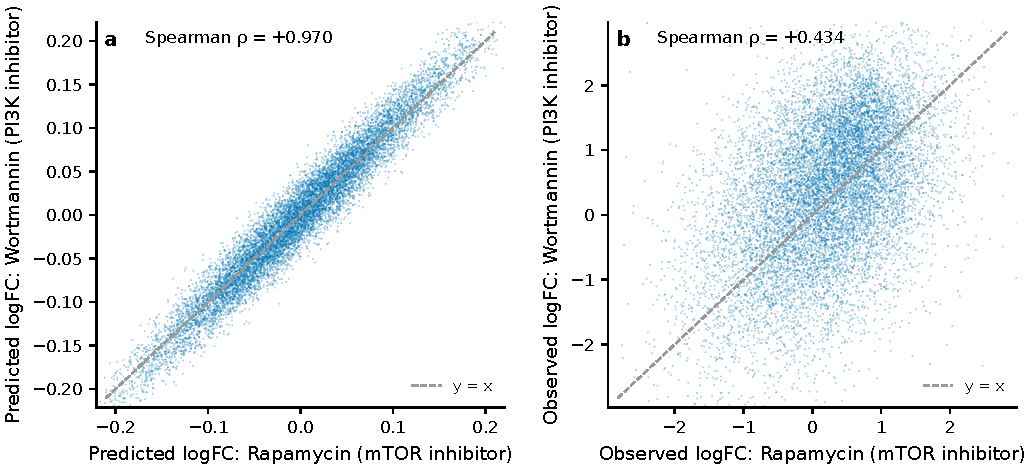
\includegraphics[width=\textwidth]{fig1_v6_correlation.pdf}
  \caption{\textbf{Transcriptome-regression collapse on opposing biological
  controls.} (\textbf{a}) Predicted log-fold-change of Rapamycin versus
  Wortmannin across all 12{,}328 genes (one point per gene; Spearman
  $\rpm=+0.970$). (\textbf{b}) Ground-truth L1000 profiles of the same two
  compounds (A549, 6\,h, highest dose; Spearman $\rpm=+0.434$). The model
  inflates the similarity between opposing pharmacologies and compresses the
  response dynamic range roughly tenfold.}
  \label{fig:collapse}
\end{figure}

\subsection*{Binary modulator classification is robust and externally valid}

Reframing the objective as binary classification (autophagy modulator versus
non-modulator) restored robust performance. For \emph{context-aware} models,
positives were 227 HAMdb modulators with matching L1000 signatures and
negatives were matched random L1000 signatures (9{,}804 train / 3{,}856 test
signatures from 137 held-out compounds; 70/30 Murcko-scaffold-aware split;
mTOR/PI3K-overlapping compounds excluded; Rapamycin and Chloroquine held out).
Morgan fingerprints consistently outperformed CLAMP embeddings here, and
XGBoost outperformed its linear ridge counterpart
(Table~\ref{tab:context}). The best context-aware model (XGBoost, Morgan +
context) reached compound-level AUROC 0.845 (compound-level probabilities are
the mean of per-signature probabilities within a compound) and AUPRC 0.810,
and ranked the held-out canonical controls at the top of the score
distribution (Rapamycin 0.981; Chloroquine 0.992).

\begin{table}[!htb]
  \centering
  \caption{\textbf{Context-aware binary modulator classification} (L1000
  signatures + cell/dose/time context; scaffold-aware held-out test of 137
  compounds). Sig., signature level.}
  \label{tab:context}
  \small
  \begin{tabular}{llccccc}
    \toprule
    Model & Features & Sig.\ AUROC & Compound AUROC & AUPRC & Rapamycin & Chloroquine \\
    \midrule
    Ridge   & Morgan + context & 0.705 & 0.823 & 0.765 & -- & -- \\
    Ridge   & CLAMP + context  & 0.560 & 0.722 & 0.654 & -- & -- \\
    XGBoost & CLAMP + context  & 0.669 & 0.800 & 0.749 & 0.706 & 0.548 \\
    XGBoost & Morgan + context & \textbf{0.765} & \textbf{0.845} & \textbf{0.810} & 0.981 & 0.992 \\
    \bottomrule
  \end{tabular}
\end{table}

Removing L1000 context entirely and training on chemical structure alone
(646 HAMdb modulators versus 5{,}893 scaffold-family-balanced ChEMBL
neutrals; 20/80 scaffold-aware split) preserved strong discrimination:
XGBoost on Morgan fingerprints reached AUROC 0.858 (AUPRC 0.642) on the
original training split, and adding CLAMP embeddings improved this slightly
(AUROC 0.866; AUPRC 0.629), the reverse of the context-aware comparison,
suggesting that CLAMP contributes bioassay-related chemical signal that is
redundant once cellular context is available.

Because single scaffold splits carry substantial sampling variance, we rebuilt
the split deterministically (\texttt{PYTHONHASHSEED}-fixed scaffold clustering,
seed 42), retrained both classifiers on the reconstructed training portion,
and evaluated them on 1{,}365 held-out compounds with 1{,}000-fold bootstrap
confidence intervals (the evaluation underlying Figure~\ref{fig:roc}):
Morgan-only AUROC 0.877 (95\% CI [0.843, 0.909]) and Morgan\,+\,CLAMP 0.839
(95\% CI [0.799, 0.875]). The intervals overlap, so on this test scale the two
models are statistically indistinguishable, in contrast to the original
split, a reminder that per-split AUROC differences of a few points should not
be over-interpreted. Consistent with this, evaluating the original saved
models (trained on a different scaffold split) on this test set inflated
AUROC to 0.97: cross-split scaffold overlap is partially memorized, which is
precisely the leakage failure mode that scaffold splitting is designed to
prevent and why models and splits must be reported jointly, with intervals.

\begin{figure}[!htb]
  \centering
  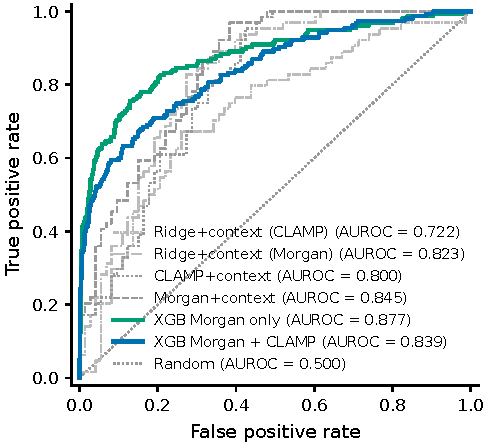
\includegraphics[width=0.62\textwidth]{fig2_binary_classifier_roc.pdf}
  \caption{\textbf{ROC curves for binary modulator classification under
  scaffold-aware validation.} Morgan fingerprints lead the context-aware
  models, and the structure-only XGBoost classifiers perform best overall
  (reconstructed evaluation split; AUROC with 95\% bootstrap intervals in
  text). Ridge baselines and the random classifier are shown for reference.}
  \label{fig:roc}
\end{figure}

\subsection*{External validation on 99{,}433 ChEMBL compounds}

We scored 99{,}433 neutral ChEMBL small molecules (deduplicated from 99{,}434
candidates; none in training) with both structure-only classifiers and
measured enrichment of orthogonal bioactivity annotations: autophagy-assay
activity and mTOR/PI3K-pathway target engagement (ChEMBL assay/target
records). Library-wide baselines are 0.18\% and 0.24\%, respectively.
Enrichment rises monotonically with score threshold for both models, with
95\% binomial confidence intervals that exclude baseline from 0.70 upward for
Morgan\,+\,CLAMP (Figure~\ref{fig:enrich}). At the most stringent threshold
($\geq0.95$; Table~\ref{tab:enrich}), Morgan\,+\,CLAMP recovers 6.41\%
autophagy-active and 13.99\% mTOR/PI3K-annotated compounds among only 343
prioritized structures (${\sim}36\times$ and ${\sim}58\times$ baseline),
outperforming Morgan-only (1.61\% and 3.23\% among 310; ${\sim}9\times$ and
${\sim}13\times$) by ${\sim}4\times$ on both axes. At this threshold the 95\%
binomial (Wilson) intervals of the two models are disjoint for both
annotation types (autophagy: [4.3, 9.5]\% versus [0.7, 3.7]\%; mTOR/PI3K:
[10.7, 18.1]\% versus [1.8, 5.8]\%), so the CLAMP-driven improvement is
statistically credible despite modest absolute counts. The top-200 hits of the
two models overlap by only 36 compounds: CLAMP shifts prioritization toward a
distinct, more biologically annotated chemical space. These enrichments are
conservative lower bounds, because many true modulators carry no ChEMBL
annotation.

\begin{table}[!htb]
  \centering
  \caption{\textbf{ChEMBL annotation enrichment at modulator-score
  thresholds.} Baselines: 0.18\% autophagy-active, 0.24\% mTOR/PI3K across
  the full library. EF, enrichment factor over the relevant baseline.}
  \label{tab:enrich}
  \footnotesize
  \begin{tabular}{cclccccc}
    \toprule
    Threshold & $n$ & Model & \% lib. & Autophagy \% & mTOR/PI3K \% &
    EF (auto.) & EF (mTOR) \\
    \midrule
    $\geq 0.50$ & 2{,}791  & Morgan+CLAMP & 2.8  & 1.61 & 3.08 & 8.9$\times$  & 12.8$\times$ \\
    $\geq 0.50$ & 21{,}897 & Morgan only  & 22.0 & 0.40 & 0.51 & 2.2$\times$  & 2.1$\times$ \\
    \midrule
    $\geq 0.80$ & 998      & Morgan+CLAMP & 1.0  & 3.31 & 6.81 & 18.4$\times$ & 28.4$\times$ \\
    $\geq 0.80$ & 4{,}314  & Morgan only  & 4.3  & 0.72 & 1.07 & 4.0$\times$  & 4.5$\times$ \\
    \midrule
    $\geq 0.95$ & 343      & Morgan+CLAMP & 0.34 & 6.41 & 13.99 & 35.6$\times$ & \textbf{58.3$\times$} \\
    $\geq 0.95$ & 310      & Morgan only  & 0.31 & 1.61 & 3.23 & 8.9$\times$  & 13.5$\times$ \\
    \bottomrule
  \end{tabular}
\end{table}

\begin{figure}[!htb]
  \centering
  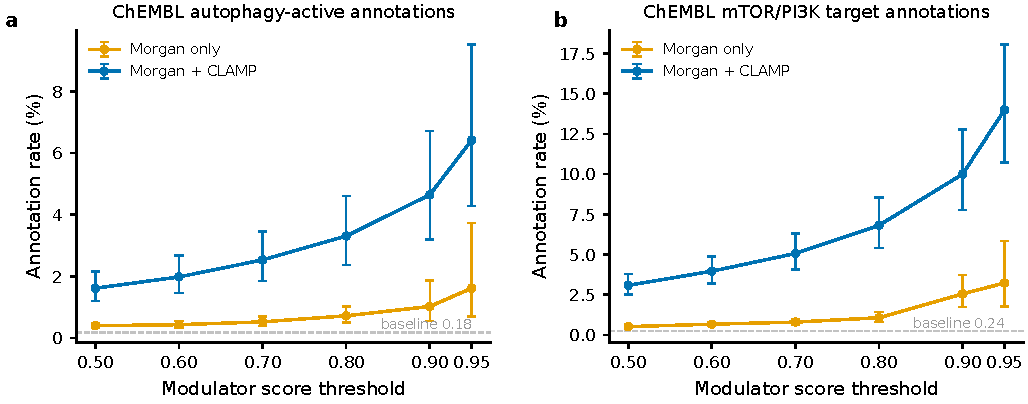
\includegraphics[width=\textwidth]{fig3_chembl_enrichment.pdf}
  \caption{\textbf{External validation on 99{,}433 ChEMBL compounds.}
  Annotation rate (a: autophagy-active; b: mTOR/PI3K pathway targets) versus
  modulator-score threshold, with 95\% binomial confidence intervals and
  library-wide baselines (dashed). Morgan\,+\,CLAMP dominates at every
  threshold, reaching 6.41\% and 13.99\% at $\geq0.95$.}
  \label{fig:enrich}
\end{figure}

\subsection*{Activator-versus-inhibitor direction prediction fails}

Binary screening succeeds; directional classification does not. A flat
3-class model (activator / inhibitor / neutral) achieved deceptively high
accuracy (0.900) but macro F1 of only 0.532 (Morgan-only) and 0.455
(Morgan\,+\,CLAMP); per-class inspection shows the score is driven almost
entirely by the dominant neutral class, with inhibitor discrimination
particularly poor (Figure~\ref{fig:multiclass}). A cascaded two-stage design
(binary screen, then a dedicated direction model) confirmed the limitation:
5-fold scaffold-aware cross-validation of the direction stage gave AUROC
$0.534\pm0.045$, AUPRC $0.366\pm0.058$, F1 $0.326\pm0.048$ (per-fold AUROCs
0.478--0.598), with held-out test AUROC 0.498, at or below random. No
representation rescued the task: class-balanced Morgan sampling was best
(AUROC $0.594\pm0.060$) and physicochemical descriptors were worse (0.454).
The two independent direction models agreed on only 55.9\% of ChEMBL
predictions.

The failure is best understood as a data problem compounded by intrinsic
ambiguity. After scaffold filtering only 132 curated inhibitors remain, an
insufficient basis for generalizable structure--direction rules, and the two
classes genuinely overlap in chemical space: lysosomotropic weak-base
inhibitors (e.g.\ Chloroquine) and kinase-targeting activators (e.g.\ mTOR
inhibitors) are not cleanly separable by substructure. Direction labels
should therefore not drive prioritization until substantially larger,
scaffold-diverse inhibitor sets exist.

\begin{figure}[!htb]
  \centering
  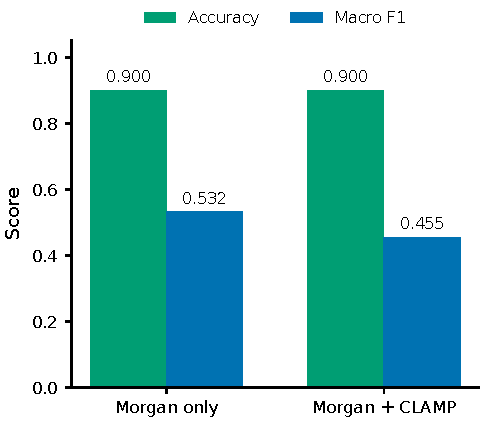
\includegraphics[width=0.55\textwidth]{fig4_multiclass_comparison.pdf}
  \caption{\textbf{Direction prediction is dominated by class imbalance.}
  Accuracy and macro F1 for flat 3-class classifiers. High accuracy reflects
  the majority neutral class; macro F1 (0.532 Morgan-only, 0.455
  Morgan\,+\,CLAMP) shows activators and inhibitors are not reliably
  separable from structure alone.}
  \label{fig:multiclass}
\end{figure}

\subsection*{Gene-signature matching captures generic stress, not autophagy flux}

As an intermediate formulation we constructed consensus autophagy signatures
(a 199-gene pathway set and a refined 25-gene flux-contrastive core; see
Methods) and ranked compounds by signature correlation. The same confounder
appeared at pathway level. An activator consensus was highly split-half
reproducible ($\rpm=0.971\pm0.006$), yet individual compound signatures
correlated with it only $0.071\pm0.270$, while \emph{random} compounds
correlated $0.713\pm0.032$: the signature largely encodes generic stress. The
inhibitor and activator consensus signatures correlated $0.63$ with each
other, consistent with compensatory autophagy transcription under lysosomal
blockade, and naive inverse search enriched random chemistry
(${\sim}15\times$ at top-50). A rigorous redesign (conservative curation,
per-cell-line contrastive signatures, dose windowing, permutation nulls,
false-discovery control) \emph{reduced} top-200 enrichment to 2--2.5\%, and
only 5 of the top 200 flux-signature hits carried ChEMBL autophagy-assay
annotations. We do not recommend signature matching for autophagy
prioritization on L1000 data.

\subsection*{What the structure-only classifier learned}

Per-bit XGBoost gains from the saved Morgan-only model (1{,}155 of 2{,}048
bits carry nonzero gain) decode to chemically plausible discriminative
environments (Figure~\ref{fig:featimp}): aliphatic amine and ether motifs
(3.3-fold enriched in modulators), diazine/purine-like heteroaromatics
(2.9-fold), thioether-linked aromatics, and an ester/acid motif (6.2-fold).
The single most enriched feature is a bare chlorine environment (10.3-fold).
High gain and high enrichment do not coincide everywhere (a
trifluoromethyl-adjacent environment ranks high by gain yet is
\emph{depleted} in modulators), showing the model exploits absence as well as
presence patterns. Because gain-based importance is biased toward
high-cardinality features and Morgan bits are hashed, these decoded SMARTS
are representative atom environments, not unique substructure assignments.

\begin{figure}[!htb]
  \centering
  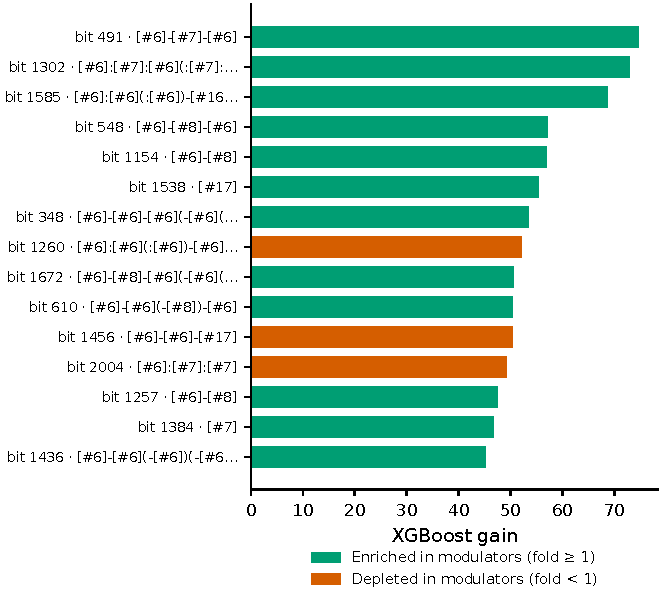
\includegraphics[width=0.6\textwidth]{fig5_feature_importance.pdf}
  \caption{\textbf{Top discriminative Morgan fingerprint bits of the
  structure-only classifier.} Bars ranked by XGBoost gain; colour encodes
  fold-enrichment of bit occurrence in modulators versus a 2{,}000-compound
  ChEMBL background (green: enriched; orange: depleted).}
  \label{fig:featimp}
\end{figure}

\section*{Discussion}

This audit's negative results are as informative as its positive ones, and
each connects to a known failure mode in the literature. The V6 collapse is a
concrete instance of what community benchmarks have begun to document for
perturbation models \cite{ahlmann2025}: high-capacity models can exhibit
smooth training dynamics while learning an invariant mean response. Our
diagnostics localize the cause upstream of architecture (no marginal
structure--expression association is detectable on a generic compound
panel) and downstream of validation methodology: the collapse was invisible
to random-split metrics and was exposed only by held-out biological controls
and by correlating the \emph{predictions} of opposing compounds. We recommend
this pairwise-control audit as standard practice for any model claiming
pathway-specific transcriptome prediction. It is also worth noting that
ground-truth opposing controls still share appreciable transcription
($\rpm=+0.43$ at 6\,h); generic stress co-occurs with real signal, which is
precisely why mean-output collapse is so easy to mistake for success.

The success of Morgan-fingerprint classifiers is consistent with
molecular-representation benchmarks in which simple fingerprints remain hard to
beat \cite{praski2025,rogers2010}. CLAMP's added value is real but
context-dependent: indistinguishable from Morgan-only on the 1{,}365-compound
held-out test, yet clearly superior at external scale on 99{,}433 ChEMBL
compounds (Figure~\ref{fig:enrich}); small held-out sets simply lack the
power to resolve differences that matter at screening scale. Two caveats
qualify the external validation.
First, CLAMP was pretrained on ChEMBL bioassay text--molecule pairs, so part
of its ChEMBL enrichment could reflect pretraining exposure rather than pure
generalization; the Morgan-only model, which shows no such overlap and still
enriches ${\sim}9$--$13\times$, provides an unaffected control. Second,
enrichment is measured against incomplete annotations; the true enrichment is
higher but unquantifiable without prospective experimental testing.

For autophagy practice, the binary modulator score is the robust output of
this pipeline. The failure of direction prediction is a data problem before
it is a modelling problem: 132 inhibitors cannot define a boundary in
fingerprint space, and lysosomotropic inhibitors and kinase-targeting
activators overlap chemically. Likewise, L1000 mRNA cannot separate autophagy
induction from lysosomal blockage \cite{klionsky2021guidelines}, and our
flux-focused signature analysis showed conserved stress responses dominate
the pathway-level signal. Future work should therefore train on direct flux
readouts (LC3-II turnover, SQSTM1/p62 degradation, lysosomal flux imaging) as
labels, expand scaffold-diverse inhibitor sets, and prospectively test the
high-confidence ChEMBL prioritizations this pipeline produces.

\section*{Methods}

\subsection*{Data resources}

\textbf{HAMdb} \cite{wang2018hamdb} provided 841 curated autophagy modulators;
after filtering to compounds with valid canonical SMILES and assignable
direction, 514 activators and 132 inhibitors (plus 167 neutral) were retained
(rule-based curation of the \texttt{Category}/pathway fields;
\texttt{hamdb\_autophagy\_directions.csv}).

\textbf{LINCS L1000 Phase I} (GSE92742; Level-5 COMPZ.MODZ,
$n473647\times12328$) \cite{subramanian2017} yielded 471{,}660 valid
signatures across 20{,}315 compounds, 5{,}509 unique Murcko scaffolds, and 76
cell lines (6--96\,h exposures). Of 813 curated HAMdb compounds, 222
(${\sim}26\%$) matched L1000 by PubChem CID; 227 modulators had usable
signatures for the context-aware task.

\textbf{Autophagy gene sets}: a 199-gene pathway set (KEGG hsa04140 +
literature) and a 25-gene flux-contrastive core (\texttt{curate\_autophagy\_genes.py}).

\textbf{ChEMBL} \cite{mendez2019}: (i) a neutral inference library of
99{,}434 candidate small molecules (99{,}433 scored after SMILES
de-duplication), pre-filtered to exclude autophagy/mTOR/PI3K/lysosomal
annotations; and (ii) assay/target annotations for enrichment analysis. A
scaffold-family-balanced subset of 5{,}893 neutrals served as training
negatives.

\subsection*{Molecular representations}

2{,}048-bit Morgan circular fingerprints (RDKit 2026.03, radius 2)
\cite{rogers2010,rdkit}; 768-dimensional CLAMP embeddings from the pretrained
checkpoint \cite{clamp}; 512-dimensional Uni-Mol 3D-aware embeddings
\cite{unimol}. Context features for L1000-context models: one-hot cell line,
$\log_{10}$ dose, one-hot exposure time.

\subsection*{Models and training}

The V6 transcriptome model was a neural network mapping Uni-Mol embeddings to
12{,}328-gene log-fold-change vectors. Classifiers used XGBoost (binary or
multi softmax objective with \texttt{scale\_pos\_weight} class balancing; up to
1{,}000 trees, depth 6) \cite{xgboost}, ridge logistic regression
(class-weighted), and multilayer perceptrons. The cascade chained the binary
Morgan-only classifier (stage 1) with a dedicated Morgan-only direction
classifier (stage 2). All random seeds were fixed (42).

\subsection*{Validation and statistics}

All splits were Murcko-scaffold-aware \cite{bemis1996,moleculenet} (context
models 70/30; structure-only 20/80) to avoid scaffold leakage
\cite{wallach2018}. Canonical controls (Rapamycin, Wortmannin, Chloroquine)
were held out and used as biological audits. Imbalanced classification was
summarized with macro F1 and precision--recall metrics rather than accuracy
alone \cite{saito2015}. Uncertainty: AUROC point estimates on the
reconstructed structure-only split are accompanied by 1{,}000-fold bootstrap
95\% confidence intervals (resampling test compounds); annotation rates carry
95\% binomial (Wilson) intervals. Enrichment factors follow early-recognition
convention \cite{truchon2007}: observed annotated fraction at threshold
divided by the library-wide baseline fraction.

\subsection*{Feature-importance analysis}

For the saved structure-only Morgan model, per-bit XGBoost gains were
decoded to atom-environment SMARTS via RDKit bit information across the 646
HAMdb modulators; fold-enrichment of bit occurrence was estimated against a
2{,}000-compound random ChEMBL background sample (seed 42).

\subsection*{Software environment}

Python 3.12; RDKit 2026.03; XGBoost 3.4.1; PyTorch 2.14 (CPU); CLAMP via its
official checkpoint; matplotlib for figures.

\section*{Data and code availability}

HAMdb: \url{http://hamdb.scbdd.com}. LINCS L1000 Phase I: GEO GSE92742.
ChEMBL: \url{https://www.ebi.ac.uk/chembl/}. {\sloppy The complete benchmarking
pipeline, trained model weights, result tables (\texttt{binary\_models\_comparison.csv},
\texttt{chembl\_enrichment\_morgan\_vs\_clamp.csv}, \texttt{paper\_feature\_importance.csv},
\texttt{bootstrap\_auroc\_ci.csv}), and figure-generation code are available
at \url{https://github.com/Abolfazl-Alipour/autophagy-modulator-prediction}
and archived at \url{https://doi.org/10.5281/zenodo.22986834}.\par}

\section*{Competing interests}

The author declares no competing interests.

\section*{Funding}

No external funding was received for this study.

\begin{thebibliography}{99}

\bibitem{levine2019}
Levine, B. \& Kroemer, G. Biological functions of autophagy genes: a disease
perspective. \textit{Cell} \textbf{176}, 11--42 (2019).
doi:10.1016/j.cell.2018.09.048

\bibitem{klionsky2021}
Klionsky, D. J. \textit{et al.} Autophagy in major human diseases.
\textit{EMBO J.} \textbf{40}, e108863 (2021).
doi:10.15252/embj.2021108863

\bibitem{galluzzi2017}
Galluzzi, L., Bravo-San Pedro, J. M., Levine, B., Green, D. R. \& Kroemer, G.
Pharmacological modulation of autophagy: therapeutic potential and persisting
obstacles. \textit{Nat. Rev. Drug Discov.} \textbf{16}, 487--511 (2017).
doi:10.1038/nrd.2017.22

\bibitem{klionsky2021guidelines}
Klionsky, D. J. \textit{et al.} Guidelines for the use and interpretation of
assays for monitoring autophagy (4th edition). \textit{Autophagy} \textbf{17},
1--382 (2021). doi:10.1080/15548627.2020.1797280

\bibitem{wang2018hamdb}
Wang, N.-N. \textit{et al.} HAMdb: a database of human autophagy modulators
with specific pathway and disease information. \textit{J. Cheminform.}
\textbf{10}, 34 (2018). doi:10.1186/s13321-018-0289-4

\bibitem{subramanian2017}
Subramanian, A. \textit{et al.} A Next Generation Connectivity Map: L1000
platform and the first 1{,}000{,}000 profiles. \textit{Cell} \textbf{171},
1437--1452 (2017). doi:10.1016/j.cell.2017.10.049

\bibitem{mendez2019}
Mendez, D. \textit{et al.} ChEMBL: towards direct deposition of bioassay
data. \textit{Nucleic Acids Res.} \textbf{47}, D930--D940 (2019).
doi:10.1093/nar/gky1075

\bibitem{dleps}
Zhu, J. \textit{et al.} Prediction of drug efficacy from transcriptional
profiles with deep learning (DLEPS). \textit{Nat. Biotechnol.} \textbf{39},
1444--1452 (2021). doi:10.1038/s41587-021-00946-z

\bibitem{deepce}
Pham, T.-H., Qiu, Y., Zeng, J., Xie, L. \& Zhang, P. A deep learning framework
for high-throughput mechanism-driven phenotype compound screening and its
application to COVID-19 drug repurposing (DeepCE). \textit{Nat. Mach. Intell.}
\textbf{3}, 247--257 (2021). doi:10.1038/s42256-020-00285-9

\bibitem{ciger}
Pham, T.-H. \textit{et al.} Chemical-induced gene expression ranking and its
application to pancreatic cancer drug repurposing (CIGER). \textit{Patterns}
\textbf{3}, 100441 (2022). doi:10.1016/j.patter.2022.100441

\bibitem{transigen}
Tong, X. \textit{et al.} Deep representation learning of chemical-induced
transcriptional profile for phenotype-based drug discovery (TranSiGen).
\textit{Nat. Commun.} \textbf{15}, 5378 (2024).
doi:10.1038/s41467-024-49620-3

\bibitem{mitcp}
Yang, K., Cheng, J., Cao, S., Pan, X., Shen, H.-B. \& Yuan, Y. Predicting
transcriptional changes induced by molecules with MiTCP. \textit{Brief.
Bioinform.} \textbf{26}, bbaf006 (2025). doi:10.1093/bib/bbaf006

\bibitem{scgen}
Lotfollahi, M., Wolf, F. A. \& Theis, F. J. scGen predicts single-cell
perturbation responses. \textit{Nat. Methods} \textbf{16}, 715--721 (2019).
doi:10.1038/s41592-019-0494-8

\bibitem{gears}
Roohani, Y., Huang, K. \& Leskovec, J. Predicting transcriptional outcomes of
novel multigene perturbations with GEARS. \textit{Nat. Biotechnol.}
\textbf{42}, 927--935 (2024). doi:10.1038/s41587-023-01905-6

\bibitem{ahlmann2025}
Ahlmann-Eltze, C., Huber, W. \& Anders, S. Deep-learning-based gene
perturbation effect prediction does not yet outperform simple linear
baselines. \textit{Nat. Methods} \textbf{22}, 1657--1661 (2025).
doi:10.1038/s41592-025-02772-6

\bibitem{praski2025}
Praski, M., Adamczyk, J. \& Czech, W. Benchmarking pretrained molecular
embedding models for molecular representation learning.
\textit{arXiv:2508.06199} (2025).

\bibitem{rogers2010}
Rogers, D. \& Hahn, M. Extended-connectivity fingerprints. \textit{J. Chem.
Inf. Model.} \textbf{50}, 742--754 (2010). doi:10.1021/ci100050t

\bibitem{unimol}
Zhou, G., Gao, Z., Ding, Q., Zheng, H., Xu, H., Wei, Z., Zhang, L. \& Ke, G.
Uni-Mol: a universal 3D molecular representation learning framework. In
\textit{Proc. 11th Int. Conf. Learning Representations (ICLR)} (2023).
OpenReview: 6K2RM6wVqKu.

\bibitem{clamp}
Seidl, P., Vall, A., Hochreiter, S. \& Klambauer, G. Enhancing activity
prediction models in drug discovery with the ability to understand human
language (CLAMP). In \textit{Proc. 40th Int. Conf. Machine Learning}, PMLR
\textbf{202}, 30458--30490 (2023).

\bibitem{xgboost}
Chen, T. \& Guestrin, C. XGBoost: a scalable tree boosting system. In
\textit{Proc. 22nd ACM SIGKDD Conf. Knowledge Discovery and Data Mining},
785--794 (2016). doi:10.1145/2939672.2939785

\bibitem{bemis1996}
Bemis, G. W. \& Murcko, M. A. The properties of known drugs. 1. Molecular
frameworks. \textit{J. Med. Chem.} \textbf{39}, 2887--2893 (1996).
doi:10.1021/jm9602928

\bibitem{moleculenet}
Wu, Z. \textit{et al.} MoleculeNet: a benchmark for molecular machine
learning. \textit{Chem. Sci.} \textbf{9}, 513--530 (2018).
doi:10.1039/C7SC02664A

\bibitem{wallach2018}
Wallach, I. \& Heifets, A. Most ligand-based classification benchmarks reward
memorization rather than generalization. \textit{J. Chem. Inf. Model.}
\textbf{58}, 916--932 (2018). doi:10.1021/acs.jcim.7b00403

\bibitem{saito2015}
Saito, T. \& Rehmsmeier, M. The precision-recall plot is more informative than
the ROC plot when evaluating binary classifiers on imbalanced datasets.
\textit{PLoS ONE} \textbf{10}, e0118432 (2015).
doi:10.1371/journal.pone.0118432

\bibitem{truchon2007}
Truchon, J.-F. \& Bayly, C. I. Evaluating virtual screening methods: good and
bad metrics for the ``early recognition'' problem. \textit{J. Chem. Inf.
Model.} \textbf{47}, 488--508 (2007). doi:10.1021/ci600426e

\bibitem{yang2024review}
Yang, Y., Pan, Z., Sun, J., Welch, J. \& Klionsky, D. J. Autophagy and machine
learning: unanswered questions. \textit{Biochim. Biophys. Acta Mol. Basis
Dis.} \textbf{1870}, 167263 (2024). doi:10.1016/j.bbadis.2024.167263

\bibitem{huang2024rw}
Huang, F., Guo, W., Chen, L., Feng, K., Huang, T. \& Cai, Y.-D. Identifying
autophagy-associated proteins and chemicals with a random walk-based method
within heterogeneous interaction network. \textit{Front. Biosci. (Landmark
Ed.)} \textbf{29}, 21 (2024). doi:10.31083/j.fbl2901021

\bibitem{rdkit}
Landrum, G. RDKit: open-source cheminformatics (software).
\url{https://www.rdkit.org}

\end{thebibliography}

\end{document}
